% Options for packages loaded elsewhere
\PassOptionsToPackage{unicode}{hyperref}
\PassOptionsToPackage{hyphens}{url}
%
\documentclass[
]{article}
\usepackage{lmodern}
\usepackage{amsmath}
\usepackage{ifxetex,ifluatex}
\ifnum 0\ifxetex 1\fi\ifluatex 1\fi=0 % if pdftex
  \usepackage[T1]{fontenc}
  \usepackage[utf8]{inputenc}
  \usepackage{textcomp} % provide euro and other symbols
  \usepackage{amssymb}
\else % if luatex or xetex
  \usepackage{unicode-math}
  \defaultfontfeatures{Scale=MatchLowercase}
  \defaultfontfeatures[\rmfamily]{Ligatures=TeX,Scale=1}
\fi
% Use upquote if available, for straight quotes in verbatim environments
\IfFileExists{upquote.sty}{\usepackage{upquote}}{}
\IfFileExists{microtype.sty}{% use microtype if available
  \usepackage[]{microtype}
  \UseMicrotypeSet[protrusion]{basicmath} % disable protrusion for tt fonts
}{}
\makeatletter
\@ifundefined{KOMAClassName}{% if non-KOMA class
  \IfFileExists{parskip.sty}{%
    \usepackage{parskip}
  }{% else
    \setlength{\parindent}{0pt}
    \setlength{\parskip}{6pt plus 2pt minus 1pt}}
}{% if KOMA class
  \KOMAoptions{parskip=half}}
\makeatother
\usepackage{xcolor}
\IfFileExists{xurl.sty}{\usepackage{xurl}}{} % add URL line breaks if available
\IfFileExists{bookmark.sty}{\usepackage{bookmark}}{\usepackage{hyperref}}
\hypersetup{
  pdftitle={CS539 hw1},
  pdfauthor={Enbo Tian},
  hidelinks,
  pdfcreator={LaTeX via pandoc}}
\urlstyle{same} % disable monospaced font for URLs
\usepackage[margin=1in]{geometry}
\usepackage{color}
\usepackage{fancyvrb}
\newcommand{\VerbBar}{|}
\newcommand{\VERB}{\Verb[commandchars=\\\{\}]}
\DefineVerbatimEnvironment{Highlighting}{Verbatim}{commandchars=\\\{\}}
% Add ',fontsize=\small' for more characters per line
\usepackage{framed}
\definecolor{shadecolor}{RGB}{248,248,248}
\newenvironment{Shaded}{\begin{snugshade}}{\end{snugshade}}
\newcommand{\AlertTok}[1]{\textcolor[rgb]{0.94,0.16,0.16}{#1}}
\newcommand{\AnnotationTok}[1]{\textcolor[rgb]{0.56,0.35,0.01}{\textbf{\textit{#1}}}}
\newcommand{\AttributeTok}[1]{\textcolor[rgb]{0.77,0.63,0.00}{#1}}
\newcommand{\BaseNTok}[1]{\textcolor[rgb]{0.00,0.00,0.81}{#1}}
\newcommand{\BuiltInTok}[1]{#1}
\newcommand{\CharTok}[1]{\textcolor[rgb]{0.31,0.60,0.02}{#1}}
\newcommand{\CommentTok}[1]{\textcolor[rgb]{0.56,0.35,0.01}{\textit{#1}}}
\newcommand{\CommentVarTok}[1]{\textcolor[rgb]{0.56,0.35,0.01}{\textbf{\textit{#1}}}}
\newcommand{\ConstantTok}[1]{\textcolor[rgb]{0.00,0.00,0.00}{#1}}
\newcommand{\ControlFlowTok}[1]{\textcolor[rgb]{0.13,0.29,0.53}{\textbf{#1}}}
\newcommand{\DataTypeTok}[1]{\textcolor[rgb]{0.13,0.29,0.53}{#1}}
\newcommand{\DecValTok}[1]{\textcolor[rgb]{0.00,0.00,0.81}{#1}}
\newcommand{\DocumentationTok}[1]{\textcolor[rgb]{0.56,0.35,0.01}{\textbf{\textit{#1}}}}
\newcommand{\ErrorTok}[1]{\textcolor[rgb]{0.64,0.00,0.00}{\textbf{#1}}}
\newcommand{\ExtensionTok}[1]{#1}
\newcommand{\FloatTok}[1]{\textcolor[rgb]{0.00,0.00,0.81}{#1}}
\newcommand{\FunctionTok}[1]{\textcolor[rgb]{0.00,0.00,0.00}{#1}}
\newcommand{\ImportTok}[1]{#1}
\newcommand{\InformationTok}[1]{\textcolor[rgb]{0.56,0.35,0.01}{\textbf{\textit{#1}}}}
\newcommand{\KeywordTok}[1]{\textcolor[rgb]{0.13,0.29,0.53}{\textbf{#1}}}
\newcommand{\NormalTok}[1]{#1}
\newcommand{\OperatorTok}[1]{\textcolor[rgb]{0.81,0.36,0.00}{\textbf{#1}}}
\newcommand{\OtherTok}[1]{\textcolor[rgb]{0.56,0.35,0.01}{#1}}
\newcommand{\PreprocessorTok}[1]{\textcolor[rgb]{0.56,0.35,0.01}{\textit{#1}}}
\newcommand{\RegionMarkerTok}[1]{#1}
\newcommand{\SpecialCharTok}[1]{\textcolor[rgb]{0.00,0.00,0.00}{#1}}
\newcommand{\SpecialStringTok}[1]{\textcolor[rgb]{0.31,0.60,0.02}{#1}}
\newcommand{\StringTok}[1]{\textcolor[rgb]{0.31,0.60,0.02}{#1}}
\newcommand{\VariableTok}[1]{\textcolor[rgb]{0.00,0.00,0.00}{#1}}
\newcommand{\VerbatimStringTok}[1]{\textcolor[rgb]{0.31,0.60,0.02}{#1}}
\newcommand{\WarningTok}[1]{\textcolor[rgb]{0.56,0.35,0.01}{\textbf{\textit{#1}}}}
\usepackage{graphicx}
\makeatletter
\def\maxwidth{\ifdim\Gin@nat@width>\linewidth\linewidth\else\Gin@nat@width\fi}
\def\maxheight{\ifdim\Gin@nat@height>\textheight\textheight\else\Gin@nat@height\fi}
\makeatother
% Scale images if necessary, so that they will not overflow the page
% margins by default, and it is still possible to overwrite the defaults
% using explicit options in \includegraphics[width, height, ...]{}
\setkeys{Gin}{width=\maxwidth,height=\maxheight,keepaspectratio}
% Set default figure placement to htbp
\makeatletter
\def\fps@figure{htbp}
\makeatother
\setlength{\emergencystretch}{3em} % prevent overfull lines
\providecommand{\tightlist}{%
  \setlength{\itemsep}{0pt}\setlength{\parskip}{0pt}}
\setcounter{secnumdepth}{-\maxdimen} % remove section numbering
\ifluatex
  \usepackage{selnolig}  % disable illegal ligatures
\fi

\title{CS539 hw1}
\author{Enbo Tian}
\date{2022/1/24}

\begin{document}
\maketitle

\hypertarget{problem-1}{%
\section{problem 1}\label{problem-1}}

\hypertarget{a}{%
\subsection{a)}\label{a}}

\begin{Shaded}
\begin{Highlighting}[]
\NormalTok{X }\OtherTok{\textless{}{-}} \FunctionTok{matrix}\NormalTok{(}\FunctionTok{runif}\NormalTok{(}\DecValTok{2} \SpecialCharTok{*} \DecValTok{2}\NormalTok{), }\DecValTok{2}\NormalTok{, }\DecValTok{2}\NormalTok{)}
\NormalTok{COV }\OtherTok{\textless{}{-}} \FunctionTok{crossprod}\NormalTok{(X)}
\NormalTok{mu }\OtherTok{\textless{}{-}} \FunctionTok{rep}\NormalTok{(}\DecValTok{0}\NormalTok{, }\DecValTok{2}\NormalTok{)}
\FunctionTok{library}\NormalTok{(MASS)}
\NormalTok{x }\OtherTok{\textless{}{-}} \FunctionTok{mvrnorm}\NormalTok{(}\DecValTok{100}\NormalTok{, mu, COV)}
\FunctionTok{plot}\NormalTok{(x)}
\end{Highlighting}
\end{Shaded}

\includegraphics{hw1_files/figure-latex/unnamed-chunk-1-1.pdf}

\hypertarget{b}{%
\section{b)}\label{b}}

\begin{Shaded}
\begin{Highlighting}[]
\NormalTok{mu }\OtherTok{\textless{}{-}} \FunctionTok{c}\NormalTok{(}\SpecialCharTok{{-}}\DecValTok{1}\NormalTok{,}\DecValTok{1}\NormalTok{)}
\NormalTok{x }\OtherTok{\textless{}{-}} \FunctionTok{mvrnorm}\NormalTok{(}\DecValTok{100}\NormalTok{, mu, COV)}
\FunctionTok{plot}\NormalTok{(x)}
\end{Highlighting}
\end{Shaded}

\includegraphics{hw1_files/figure-latex/unnamed-chunk-2-1.pdf}

\begin{Shaded}
\begin{Highlighting}[]
\NormalTok{mu }\OtherTok{\textless{}{-}} \FunctionTok{c}\NormalTok{(}\DecValTok{0}\NormalTok{,}\DecValTok{0}\NormalTok{)}
\end{Highlighting}
\end{Shaded}

The interval of x1 is moving left by about 1, and the interval of x2 is
moving up by about 1.

\hypertarget{c}{%
\subsection{c)}\label{c}}

\begin{Shaded}
\begin{Highlighting}[]
\NormalTok{COV }\OtherTok{\textless{}{-}} \DecValTok{2}\SpecialCharTok{*}\NormalTok{COV}
\NormalTok{x }\OtherTok{\textless{}{-}} \FunctionTok{mvrnorm}\NormalTok{(}\DecValTok{100}\NormalTok{, mu, COV)}
\FunctionTok{plot}\NormalTok{(x)}
\end{Highlighting}
\end{Shaded}

\includegraphics{hw1_files/figure-latex/unnamed-chunk-3-1.pdf}

\hypertarget{d}{%
\subsection{d)}\label{d}}

\begin{Shaded}
\begin{Highlighting}[]
\NormalTok{COV }\OtherTok{\textless{}{-}} \FunctionTok{matrix}\NormalTok{(}\FunctionTok{c}\NormalTok{(}\DecValTok{1}\NormalTok{,}\FloatTok{0.5}\NormalTok{,}\FloatTok{0.5}\NormalTok{,}\DecValTok{1}\NormalTok{), }\AttributeTok{nrow =} \DecValTok{2}\NormalTok{, }\AttributeTok{ncol =} \DecValTok{2}\NormalTok{)}
\NormalTok{x }\OtherTok{\textless{}{-}} \FunctionTok{mvrnorm}\NormalTok{(}\DecValTok{100}\NormalTok{, mu, COV)}
\FunctionTok{plot}\NormalTok{(x)}
\end{Highlighting}
\end{Shaded}

\includegraphics{hw1_files/figure-latex/unnamed-chunk-4-1.pdf}

\hypertarget{e}{%
\subsection{e)}\label{e}}

\begin{Shaded}
\begin{Highlighting}[]
\NormalTok{COV }\OtherTok{\textless{}{-}} \FunctionTok{matrix}\NormalTok{(}\FunctionTok{c}\NormalTok{(}\DecValTok{1}\NormalTok{,}\SpecialCharTok{{-}}\FloatTok{0.5}\NormalTok{,}\SpecialCharTok{{-}}\FloatTok{0.5}\NormalTok{,}\DecValTok{1}\NormalTok{), }\AttributeTok{nrow =} \DecValTok{2}\NormalTok{, }\AttributeTok{ncol =} \DecValTok{2}\NormalTok{)}
\NormalTok{x }\OtherTok{\textless{}{-}} \FunctionTok{mvrnorm}\NormalTok{(}\DecValTok{100}\NormalTok{, mu, COV)}
\FunctionTok{plot}\NormalTok{(x)}
\end{Highlighting}
\end{Shaded}

\includegraphics{hw1_files/figure-latex/unnamed-chunk-5-1.pdf}

\hypertarget{f}{%
\subsection{f)}\label{f}}

\begin{Shaded}
\begin{Highlighting}[]
\NormalTok{X }\OtherTok{\textless{}{-}} \FunctionTok{matrix}\NormalTok{(}\FunctionTok{runif}\NormalTok{(}\DecValTok{2} \SpecialCharTok{*} \DecValTok{2}\NormalTok{), }\DecValTok{2}\NormalTok{, }\DecValTok{2}\NormalTok{)}
\NormalTok{COV }\OtherTok{\textless{}{-}} \FunctionTok{crossprod}\NormalTok{(X)}
\NormalTok{mu }\OtherTok{\textless{}{-}} \FunctionTok{rep}\NormalTok{(}\DecValTok{0}\NormalTok{, }\DecValTok{2}\NormalTok{)}
\NormalTok{x }\OtherTok{\textless{}{-}} \FunctionTok{mvrnorm}\NormalTok{(}\DecValTok{100}\NormalTok{, mu, COV)}
\FunctionTok{mean}\NormalTok{(x)}
\end{Highlighting}
\end{Shaded}

\begin{verbatim}
## [1] 0.01085692
\end{verbatim}

\begin{Shaded}
\begin{Highlighting}[]
\FunctionTok{cov}\NormalTok{(x)}
\end{Highlighting}
\end{Shaded}

\begin{verbatim}
##           [,1]      [,2]
## [1,] 0.3256741 0.5444007
## [2,] 0.5444007 0.9690941
\end{verbatim}

\hypertarget{g}{%
\subsection{g)}\label{g}}

\begin{Shaded}
\begin{Highlighting}[]
\NormalTok{COV }\OtherTok{\textless{}{-}} \FunctionTok{matrix}\NormalTok{(}\FunctionTok{c}\NormalTok{(}\DecValTok{1}\NormalTok{,}\SpecialCharTok{{-}}\FloatTok{0.5}\NormalTok{,}\SpecialCharTok{{-}}\FloatTok{0.5}\NormalTok{,}\DecValTok{1}\NormalTok{), }\AttributeTok{nrow =} \DecValTok{2}\NormalTok{, }\AttributeTok{ncol =} \DecValTok{2}\NormalTok{)}
\NormalTok{x }\OtherTok{\textless{}{-}} \FunctionTok{mvrnorm}\NormalTok{(}\DecValTok{1000}\NormalTok{, mu, COV)}
\FunctionTok{plot}\NormalTok{(x)}
\end{Highlighting}
\end{Shaded}

\includegraphics{hw1_files/figure-latex/unnamed-chunk-7-1.pdf}

\hypertarget{h}{%
\subsection{h)}\label{h}}

\begin{Shaded}
\begin{Highlighting}[]
\FunctionTok{mean}\NormalTok{(x)}
\end{Highlighting}
\end{Shaded}

\begin{verbatim}
## [1] 0.01001381
\end{verbatim}

\begin{Shaded}
\begin{Highlighting}[]
\FunctionTok{cov}\NormalTok{(x)}
\end{Highlighting}
\end{Shaded}

\begin{verbatim}
##            [,1]       [,2]
## [1,]  1.0034878 -0.4993829
## [2,] -0.4993829  0.9456714
\end{verbatim}

\hypertarget{i}{%
\subsection{i)}\label{i}}

\begin{Shaded}
\begin{Highlighting}[]
\NormalTok{x }\OtherTok{\textless{}{-}} \FunctionTok{mvrnorm}\NormalTok{(}\DecValTok{10}\NormalTok{, mu, COV)}
\FunctionTok{mean}\NormalTok{(x[,}\DecValTok{1}\NormalTok{])}
\end{Highlighting}
\end{Shaded}

\begin{verbatim}
## [1] -0.5509923
\end{verbatim}

\begin{Shaded}
\begin{Highlighting}[]
\NormalTok{x }\OtherTok{\textless{}{-}} \FunctionTok{mvrnorm}\NormalTok{(}\DecValTok{100}\NormalTok{, mu, COV)}
\FunctionTok{mean}\NormalTok{(x[,}\DecValTok{1}\NormalTok{])}
\end{Highlighting}
\end{Shaded}

\begin{verbatim}
## [1] -0.02584581
\end{verbatim}

\begin{Shaded}
\begin{Highlighting}[]
\NormalTok{x }\OtherTok{\textless{}{-}} \FunctionTok{mvrnorm}\NormalTok{(}\DecValTok{1000}\NormalTok{, mu, COV)}
\FunctionTok{mean}\NormalTok{(x[,}\DecValTok{1}\NormalTok{])}
\end{Highlighting}
\end{Shaded}

\begin{verbatim}
## [1] -0.01481128
\end{verbatim}

Mean is tend to 0, as the more samples we have

\hypertarget{j}{%
\subsection{j)}\label{j}}

\begin{Shaded}
\begin{Highlighting}[]
\NormalTok{COV }\CommentTok{\# the initial covariance we use to get the sample}
\end{Highlighting}
\end{Shaded}

\begin{verbatim}
##      [,1] [,2]
## [1,]  1.0 -0.5
## [2,] -0.5  1.0
\end{verbatim}

\begin{Shaded}
\begin{Highlighting}[]
\NormalTok{x }\OtherTok{\textless{}{-}} \FunctionTok{mvrnorm}\NormalTok{(}\DecValTok{10}\NormalTok{, mu, COV)}
\FunctionTok{cov}\NormalTok{(x)}
\end{Highlighting}
\end{Shaded}

\begin{verbatim}
##            [,1]       [,2]
## [1,]  1.0542073 -0.1427236
## [2,] -0.1427236  0.7384374
\end{verbatim}

\begin{Shaded}
\begin{Highlighting}[]
\NormalTok{x }\OtherTok{\textless{}{-}} \FunctionTok{mvrnorm}\NormalTok{(}\DecValTok{100}\NormalTok{, mu, COV)}
\FunctionTok{cov}\NormalTok{(x)}
\end{Highlighting}
\end{Shaded}

\begin{verbatim}
##            [,1]       [,2]
## [1,]  1.1167154 -0.5027765
## [2,] -0.5027765  0.9957042
\end{verbatim}

\begin{Shaded}
\begin{Highlighting}[]
\NormalTok{x }\OtherTok{\textless{}{-}} \FunctionTok{mvrnorm}\NormalTok{(}\DecValTok{1000}\NormalTok{, mu, COV)}
\FunctionTok{cov}\NormalTok{(x)}
\end{Highlighting}
\end{Shaded}

\begin{verbatim}
##            [,1]       [,2]
## [1,]  1.0245853 -0.5510403
## [2,] -0.5510403  1.1533854
\end{verbatim}

covariance is getting closer to the initial covariance, When we have
more sample

\hypertarget{problem-2}{%
\section{problem 2}\label{problem-2}}

\hypertarget{a-1}{%
\subsection{a)}\label{a-1}}

\begin{Shaded}
\begin{Highlighting}[]
\NormalTok{class1 }\OtherTok{\textless{}{-}} \FunctionTok{rnorm}\NormalTok{(}\DecValTok{1000}\NormalTok{,}\SpecialCharTok{{-}}\DecValTok{1}\NormalTok{,}\DecValTok{1}\NormalTok{)}
\end{Highlighting}
\end{Shaded}

\hypertarget{b-1}{%
\subsection{b)}\label{b-1}}

\begin{Shaded}
\begin{Highlighting}[]
\NormalTok{class2 }\OtherTok{\textless{}{-}} \FunctionTok{rnorm}\NormalTok{(}\DecValTok{1000}\NormalTok{,}\DecValTok{2}\NormalTok{,}\DecValTok{2}\NormalTok{)}
\end{Highlighting}
\end{Shaded}

\hypertarget{c-1}{%
\subsection{c)}\label{c-1}}

\begin{Shaded}
\begin{Highlighting}[]
\FunctionTok{hist}\NormalTok{(class1, }\AttributeTok{col=}\StringTok{\textquotesingle{}red\textquotesingle{}}\NormalTok{)}
\FunctionTok{hist}\NormalTok{(class2, }\AttributeTok{col=}\StringTok{\textquotesingle{}blue\textquotesingle{}}\NormalTok{, }\AttributeTok{add=}\ConstantTok{TRUE}\NormalTok{)}
\end{Highlighting}
\end{Shaded}

\includegraphics{hw1_files/figure-latex/unnamed-chunk-13-1.pdf}

\hypertarget{d-1}{%
\subsection{d)}\label{d-1}}

\begin{Shaded}
\begin{Highlighting}[]
\FunctionTok{library}\NormalTok{(stats4)}
\FunctionTok{library}\NormalTok{(methods)}
\FunctionTok{options}\NormalTok{(}\AttributeTok{warn =} \SpecialCharTok{{-}}\DecValTok{1}\NormalTok{)}
\NormalTok{LL1 }\OtherTok{\textless{}{-}} \ControlFlowTok{function}\NormalTok{(mu,sigma)\{}
  \SpecialCharTok{{-}}\FunctionTok{sum}\NormalTok{(}\FunctionTok{log}\NormalTok{(}\FunctionTok{dnorm}\NormalTok{(class1,mu,sigma)))}
\NormalTok{\}}
\NormalTok{m1}\OtherTok{\textless{}{-}}\FunctionTok{mle}\NormalTok{(LL1,}\AttributeTok{start =} \FunctionTok{list}\NormalTok{(}\AttributeTok{mu=}\DecValTok{0}\NormalTok{,}\AttributeTok{sigma=}\DecValTok{1}\NormalTok{))}
\NormalTok{m1}
\end{Highlighting}
\end{Shaded}

\begin{verbatim}
## 
## Call:
## mle(minuslogl = LL1, start = list(mu = 0, sigma = 1))
## 
## Coefficients:
##         mu      sigma 
## -0.9885079  0.9712683
\end{verbatim}

\begin{Shaded}
\begin{Highlighting}[]
\NormalTok{LL2 }\OtherTok{\textless{}{-}} \ControlFlowTok{function}\NormalTok{(mu,sigma)\{}
\NormalTok{  R }\OtherTok{=} \FunctionTok{dnorm}\NormalTok{(class2,mu,sigma)}
  \SpecialCharTok{{-}}\FunctionTok{sum}\NormalTok{(}\FunctionTok{log}\NormalTok{(R))}
\NormalTok{\}}
\NormalTok{m2}\OtherTok{\textless{}{-}}\FunctionTok{mle}\NormalTok{(LL2,}\AttributeTok{start =} \FunctionTok{list}\NormalTok{(}\AttributeTok{mu=}\DecValTok{0}\NormalTok{,}\AttributeTok{sigma=}\DecValTok{1}\NormalTok{))}
\NormalTok{m2}
\end{Highlighting}
\end{Shaded}

\begin{verbatim}
## 
## Call:
## mle(minuslogl = LL2, start = list(mu = 0, sigma = 1))
## 
## Coefficients:
##       mu    sigma 
## 1.966136 1.959162
\end{verbatim}

\begin{Shaded}
\begin{Highlighting}[]
\FunctionTok{options}\NormalTok{(}\AttributeTok{warn =} \FunctionTok{getOption}\NormalTok{(}\StringTok{"warn"}\NormalTok{))}
\end{Highlighting}
\end{Shaded}

\hypertarget{e-1}{%
\subsection{e)}\label{e-1}}

\begin{Shaded}
\begin{Highlighting}[]
\NormalTok{mu1 }\OtherTok{\textless{}{-}}\NormalTok{ m1}\SpecialCharTok{@}\NormalTok{coef[}\DecValTok{1}\NormalTok{]}
\NormalTok{sigma1}\OtherTok{\textless{}{-}}\NormalTok{ m1}\SpecialCharTok{@}\NormalTok{coef[}\DecValTok{2}\NormalTok{]}
\NormalTok{mu2}\OtherTok{\textless{}{-}}\NormalTok{m2}\SpecialCharTok{@}\NormalTok{coef[}\DecValTok{1}\NormalTok{]}
\NormalTok{sigma2}\OtherTok{\textless{}{-}}\NormalTok{m2}\SpecialCharTok{@}\NormalTok{coef[}\DecValTok{2}\NormalTok{]}

\NormalTok{x }\OtherTok{\textless{}{-}} \FunctionTok{seq}\NormalTok{(}\SpecialCharTok{{-}}\DecValTok{10}\NormalTok{, }\DecValTok{10}\NormalTok{, }\AttributeTok{length=}\DecValTok{100}\NormalTok{)}
\FunctionTok{plot}\NormalTok{(x,}\FunctionTok{dnorm}\NormalTok{(x,mu1,sigma1), }\AttributeTok{type =} \StringTok{"l"}\NormalTok{,}\AttributeTok{col =} \StringTok{"red"}\NormalTok{)}
\FunctionTok{par}\NormalTok{(}\AttributeTok{new=}\ConstantTok{TRUE}\NormalTok{)}
\FunctionTok{plot}\NormalTok{(x,}\FunctionTok{dnorm}\NormalTok{(x,mu2,sigma2), }\AttributeTok{type =} \StringTok{"l"}\NormalTok{,}\AttributeTok{col=}\StringTok{"blue"}\NormalTok{)}
\NormalTok{i }\OtherTok{=} \SpecialCharTok{{-}}\DecValTok{2}
\ControlFlowTok{while}\NormalTok{(}\FunctionTok{round}\NormalTok{(}\FunctionTok{dnorm}\NormalTok{(i,mu1,sigma1),}\DecValTok{5}\NormalTok{)}\SpecialCharTok{!=}\FunctionTok{round}\NormalTok{(}\FunctionTok{dnorm}\NormalTok{(i,mu2,sigma2),}\DecValTok{5}\NormalTok{))\{}
\NormalTok{  i}\OtherTok{=}\NormalTok{i}\FloatTok{+0.00001}
\NormalTok{\}}
\FunctionTok{par}\NormalTok{(}\AttributeTok{new=}\ConstantTok{TRUE}\NormalTok{)}
\FunctionTok{abline}\NormalTok{(}\AttributeTok{v=}\SpecialCharTok{{-}}\FloatTok{0.014}\NormalTok{)}
\end{Highlighting}
\end{Shaded}

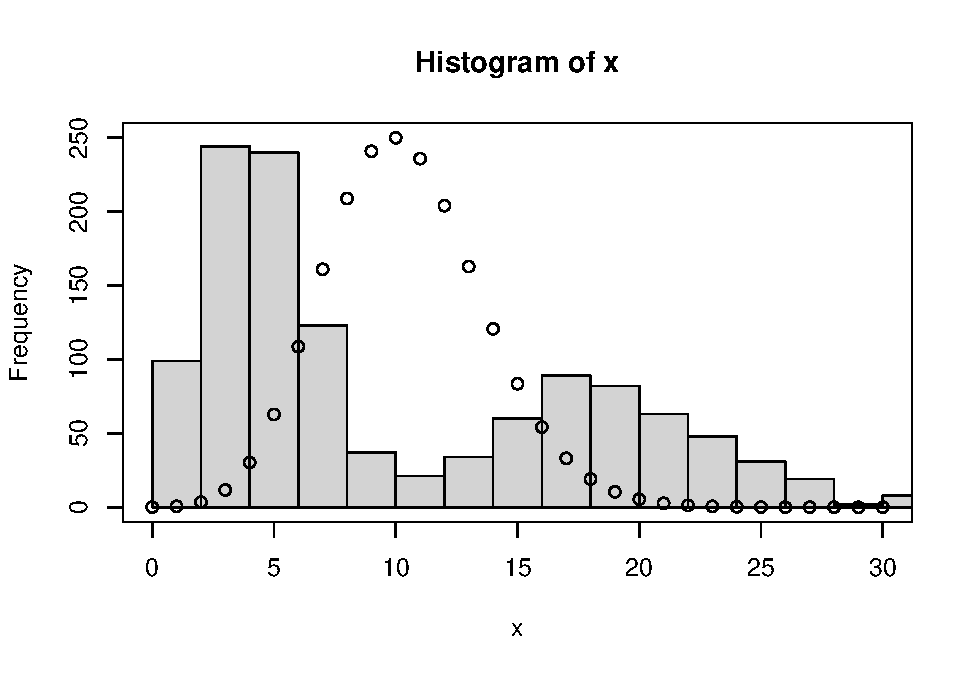
\includegraphics{hw1_files/figure-latex/unnamed-chunk-15-1.pdf}

\hypertarget{f-1}{%
\subsection{f)}\label{f-1}}

both of the decision boundary of pdf and histogram are about 0

\hypertarget{g-1}{%
\subsection{g)}\label{g-1}}

\begin{Shaded}
\begin{Highlighting}[]
\NormalTok{class2 }\OtherTok{\textless{}{-}} \FunctionTok{rnorm}\NormalTok{(}\DecValTok{2000}\NormalTok{,}\DecValTok{2}\NormalTok{,}\DecValTok{2}\NormalTok{)}
\CommentTok{\#c}
\FunctionTok{hist}\NormalTok{(class1, }\AttributeTok{col=}\StringTok{\textquotesingle{}red\textquotesingle{}}\NormalTok{)}
\FunctionTok{hist}\NormalTok{(class2, }\AttributeTok{col=}\StringTok{\textquotesingle{}blue\textquotesingle{}}\NormalTok{, }\AttributeTok{add=}\ConstantTok{TRUE}\NormalTok{)}
\end{Highlighting}
\end{Shaded}

\includegraphics{hw1_files/figure-latex/unnamed-chunk-16-1.pdf}

\begin{Shaded}
\begin{Highlighting}[]
\CommentTok{\#d}
\FunctionTok{options}\NormalTok{(}\AttributeTok{warn =} \SpecialCharTok{{-}}\DecValTok{1}\NormalTok{)}
\NormalTok{LL1 }\OtherTok{\textless{}{-}} \ControlFlowTok{function}\NormalTok{(mu,sigma)\{}
  \SpecialCharTok{{-}}\FunctionTok{sum}\NormalTok{(}\FunctionTok{log}\NormalTok{(}\FunctionTok{dnorm}\NormalTok{(class1,mu,sigma)))}
\NormalTok{\}}
\NormalTok{m1}\OtherTok{\textless{}{-}}\FunctionTok{mle}\NormalTok{(LL1,}\AttributeTok{start =} \FunctionTok{list}\NormalTok{(}\AttributeTok{mu=}\DecValTok{0}\NormalTok{,}\AttributeTok{sigma=}\DecValTok{1}\NormalTok{))}
\NormalTok{m1}
\end{Highlighting}
\end{Shaded}

\begin{verbatim}
## 
## Call:
## mle(minuslogl = LL1, start = list(mu = 0, sigma = 1))
## 
## Coefficients:
##         mu      sigma 
## -0.9885079  0.9712683
\end{verbatim}

\begin{Shaded}
\begin{Highlighting}[]
\NormalTok{LL2 }\OtherTok{\textless{}{-}} \ControlFlowTok{function}\NormalTok{(mu,sigma)\{}
\NormalTok{  R }\OtherTok{=} \FunctionTok{dnorm}\NormalTok{(class2,mu,sigma)}
  \SpecialCharTok{{-}}\FunctionTok{sum}\NormalTok{(}\FunctionTok{log}\NormalTok{(R))}
\NormalTok{\}}
\NormalTok{m2}\OtherTok{\textless{}{-}}\FunctionTok{mle}\NormalTok{(LL2,}\AttributeTok{start =} \FunctionTok{list}\NormalTok{(}\AttributeTok{mu=}\DecValTok{0}\NormalTok{,}\AttributeTok{sigma=}\DecValTok{1}\NormalTok{))}
\NormalTok{m2}
\end{Highlighting}
\end{Shaded}

\begin{verbatim}
## 
## Call:
## mle(minuslogl = LL2, start = list(mu = 0, sigma = 1))
## 
## Coefficients:
##       mu    sigma 
## 1.991904 2.036327
\end{verbatim}

\begin{Shaded}
\begin{Highlighting}[]
\FunctionTok{options}\NormalTok{(}\AttributeTok{warn =} \FunctionTok{getOption}\NormalTok{(}\StringTok{"warn"}\NormalTok{))}
\CommentTok{\#e}
\NormalTok{mu1 }\OtherTok{\textless{}{-}}\NormalTok{ m1}\SpecialCharTok{@}\NormalTok{coef[}\DecValTok{1}\NormalTok{]}
\NormalTok{sigma1}\OtherTok{\textless{}{-}}\NormalTok{ m1}\SpecialCharTok{@}\NormalTok{coef[}\DecValTok{2}\NormalTok{]}
\NormalTok{mu2}\OtherTok{\textless{}{-}}\NormalTok{m2}\SpecialCharTok{@}\NormalTok{coef[}\DecValTok{1}\NormalTok{]}
\NormalTok{sigma2}\OtherTok{\textless{}{-}}\NormalTok{m2}\SpecialCharTok{@}\NormalTok{coef[}\DecValTok{2}\NormalTok{]}

\NormalTok{x }\OtherTok{\textless{}{-}} \FunctionTok{seq}\NormalTok{(}\SpecialCharTok{{-}}\DecValTok{10}\NormalTok{, }\DecValTok{10}\NormalTok{, }\AttributeTok{length=}\DecValTok{100}\NormalTok{)}
\FunctionTok{plot}\NormalTok{(x,}\FunctionTok{dnorm}\NormalTok{(x,mu1,sigma1), }\AttributeTok{type =} \StringTok{"l"}\NormalTok{,}\AttributeTok{col =} \StringTok{"red"}\NormalTok{)}
\FunctionTok{par}\NormalTok{(}\AttributeTok{new=}\ConstantTok{TRUE}\NormalTok{)}
\FunctionTok{plot}\NormalTok{(x,}\FunctionTok{dnorm}\NormalTok{(x,mu2,sigma2), }\AttributeTok{type =} \StringTok{"l"}\NormalTok{,}\AttributeTok{col=}\StringTok{"blue"}\NormalTok{)}
\NormalTok{i }\OtherTok{=} \SpecialCharTok{{-}}\DecValTok{2}
\ControlFlowTok{while}\NormalTok{(}\FunctionTok{round}\NormalTok{(}\FunctionTok{dnorm}\NormalTok{(i,mu1,sigma1),}\DecValTok{5}\NormalTok{)}\SpecialCharTok{!=}\FunctionTok{round}\NormalTok{(}\FunctionTok{dnorm}\NormalTok{(i,mu2,sigma2),}\DecValTok{5}\NormalTok{))\{}
\NormalTok{  i}\OtherTok{=}\NormalTok{i}\FloatTok{+0.0001}
\NormalTok{\}}
\FunctionTok{par}\NormalTok{(}\AttributeTok{new=}\ConstantTok{TRUE}\NormalTok{)}
\FunctionTok{abline}\NormalTok{(}\AttributeTok{v=}\SpecialCharTok{{-}}\FloatTok{0.016}\NormalTok{)}
\end{Highlighting}
\end{Shaded}

\includegraphics{hw1_files/figure-latex/unnamed-chunk-16-2.pdf}

\begin{Shaded}
\begin{Highlighting}[]
\CommentTok{\#f}
\end{Highlighting}
\end{Shaded}

Since there are more samples in class2, the decision boundary of
histogram comes to -1, but the decision boundary of pdf does not change.

\hypertarget{h-1}{%
\subsection{h)}\label{h-1}}

\begin{Shaded}
\begin{Highlighting}[]
\FunctionTok{library}\NormalTok{(MASS)}
\FunctionTok{fitdistr}\NormalTok{(class1, }\AttributeTok{densfun=}\StringTok{"normal"}\NormalTok{)}
\end{Highlighting}
\end{Shaded}

\begin{verbatim}
##       mean           sd     
##   -0.98849358    0.97124399 
##  ( 0.03071343) ( 0.02171768)
\end{verbatim}

\begin{Shaded}
\begin{Highlighting}[]
\NormalTok{class2 }\OtherTok{\textless{}{-}} \FunctionTok{rnorm}\NormalTok{(}\DecValTok{1000}\NormalTok{,}\DecValTok{2}\NormalTok{,}\DecValTok{2}\NormalTok{)}
\FunctionTok{fitdistr}\NormalTok{(class2, }\AttributeTok{densfun=}\StringTok{"normal"}\NormalTok{)}
\end{Highlighting}
\end{Shaded}

\begin{verbatim}
##       mean          sd    
##   2.04589578   2.01786866 
##  (0.06381061) (0.04512091)
\end{verbatim}

the error rate are on the second line.

\begin{Shaded}
\begin{Highlighting}[]
\FunctionTok{library}\NormalTok{(MASS)}
\FunctionTok{fitdistr}\NormalTok{(class1, }\AttributeTok{densfun=}\StringTok{"normal"}\NormalTok{)}
\end{Highlighting}
\end{Shaded}

\begin{verbatim}
##       mean           sd     
##   -0.98849358    0.97124399 
##  ( 0.03071343) ( 0.02171768)
\end{verbatim}

\begin{Shaded}
\begin{Highlighting}[]
\NormalTok{class2 }\OtherTok{\textless{}{-}} \FunctionTok{rnorm}\NormalTok{(}\DecValTok{2000}\NormalTok{,}\DecValTok{2}\NormalTok{,}\DecValTok{2}\NormalTok{)}
\FunctionTok{fitdistr}\NormalTok{(class2, }\AttributeTok{densfun=}\StringTok{"normal"}\NormalTok{)}
\end{Highlighting}
\end{Shaded}

\begin{verbatim}
##       mean          sd    
##   2.01881882   1.97356733 
##  (0.04413031) (0.03120484)
\end{verbatim}

\hypertarget{i-1}{%
\subsection{i)}\label{i-1}}

\begin{Shaded}
\begin{Highlighting}[]
\FunctionTok{options}\NormalTok{(}\AttributeTok{warn =} \SpecialCharTok{{-}}\DecValTok{1}\NormalTok{)}
\NormalTok{df }\OtherTok{\textless{}{-}} \FunctionTok{data.frame}\NormalTok{(class1,class2)}
\FunctionTok{library}\NormalTok{(pROC)}
\end{Highlighting}
\end{Shaded}

\begin{verbatim}
## Type 'citation("pROC")' for a citation.
\end{verbatim}

\begin{verbatim}
## 
## 载入程辑包:'pROC'
\end{verbatim}

\begin{verbatim}
## The following objects are masked from 'package:stats':
## 
##     cov, smooth, var
\end{verbatim}

\begin{Shaded}
\begin{Highlighting}[]
\FunctionTok{roc}\NormalTok{(df}\SpecialCharTok{$}\NormalTok{class1,df}\SpecialCharTok{$}\NormalTok{class2,}\AttributeTok{plot=}\ConstantTok{TRUE}\NormalTok{)}
\end{Highlighting}
\end{Shaded}

\begin{verbatim}
## Setting levels: control = -4.31209473537503, case = -4.1727696341978
\end{verbatim}

\begin{verbatim}
## Setting direction: controls < cases
\end{verbatim}

\includegraphics{hw1_files/figure-latex/unnamed-chunk-19-1.pdf}

\begin{verbatim}
## 
## Call:
## roc.default(response = df$class1, predictor = df$class2, plot = TRUE)
## 
## Data: df$class2 in 2 controls (df$class1 -4.31209473537503) < 2 cases (df$class1 -4.1727696341978).
## Area under the curve: 0.75
\end{verbatim}

\begin{Shaded}
\begin{Highlighting}[]
\FunctionTok{options}\NormalTok{(}\AttributeTok{warn =} \FunctionTok{getOption}\NormalTok{(}\StringTok{"warn"}\NormalTok{))}
\end{Highlighting}
\end{Shaded}

\hypertarget{problem-3}{%
\section{problem 3}\label{problem-3}}

\hypertarget{a-2}{%
\subsection{a)}\label{a-2}}

\begin{Shaded}
\begin{Highlighting}[]
\FunctionTok{library}\NormalTok{(}\StringTok{"Rlab"}\NormalTok{) }
\end{Highlighting}
\end{Shaded}

\begin{verbatim}
## Rlab 2.15.1 attached.
\end{verbatim}

\begin{verbatim}
## 
## 载入程辑包:'Rlab'
\end{verbatim}

\begin{verbatim}
## The following object is masked from 'package:MASS':
## 
##     michelson
\end{verbatim}

\begin{verbatim}
## The following objects are masked from 'package:stats':
## 
##     dexp, dgamma, dweibull, pexp, pgamma, pweibull, qexp, qgamma,
##     qweibull, rexp, rgamma, rweibull
\end{verbatim}

\begin{verbatim}
## The following object is masked from 'package:datasets':
## 
##     precip
\end{verbatim}

\begin{Shaded}
\begin{Highlighting}[]
\NormalTok{coin }\OtherTok{\textless{}{-}} \FunctionTok{rbern}\NormalTok{(}\DecValTok{1000}\NormalTok{, }\FloatTok{0.6}\NormalTok{)}
\end{Highlighting}
\end{Shaded}

\#\#b)

\begin{Shaded}
\begin{Highlighting}[]
\FunctionTok{options}\NormalTok{(}\AttributeTok{warn =} \SpecialCharTok{{-}}\DecValTok{1}\NormalTok{)}
\NormalTok{LL1 }\OtherTok{\textless{}{-}} \ControlFlowTok{function}\NormalTok{(p)\{}
  \SpecialCharTok{{-}}\FunctionTok{sum}\NormalTok{(}\FunctionTok{log}\NormalTok{(}\FunctionTok{dbern}\NormalTok{(coin,p)))}
\NormalTok{\}}
\NormalTok{m1}\OtherTok{\textless{}{-}}\FunctionTok{mle}\NormalTok{(LL1,}\AttributeTok{start =} \FunctionTok{list}\NormalTok{(}\AttributeTok{p=}\FloatTok{0.01}\NormalTok{))}
\NormalTok{m1}\SpecialCharTok{@}\NormalTok{coef}
\end{Highlighting}
\end{Shaded}

\begin{verbatim}
##         p 
## 0.5729984
\end{verbatim}

\begin{Shaded}
\begin{Highlighting}[]
\NormalTok{LL }\OtherTok{\textless{}{-}} \ControlFlowTok{function}\NormalTok{(n,p)\{}
  \SpecialCharTok{{-}}\FunctionTok{sum}\NormalTok{(}\FunctionTok{log}\NormalTok{(}\FunctionTok{dbern}\NormalTok{(}\FunctionTok{rbern}\NormalTok{(n, }\FloatTok{0.6}\NormalTok{),p)))}
\NormalTok{\}}

\ControlFlowTok{for}\NormalTok{(n }\ControlFlowTok{in} \DecValTok{1}\SpecialCharTok{:}\DecValTok{1000}\NormalTok{)\{}
\NormalTok{  ll }\OtherTok{\textless{}{-}} \ControlFlowTok{function}\NormalTok{(p)\{}
    \FunctionTok{LL}\NormalTok{(n,p)}
\NormalTok{  \}}
\NormalTok{  m1}\OtherTok{\textless{}{-}}\FunctionTok{mle}\NormalTok{(LL1,}\AttributeTok{start =} \FunctionTok{list}\NormalTok{(}\AttributeTok{p=}\FloatTok{0.01}\NormalTok{))}
\NormalTok{  pi[n]}\OtherTok{\textless{}{-}}\NormalTok{m1}\SpecialCharTok{@}\NormalTok{coef}
\NormalTok{\}}

\NormalTok{x}\OtherTok{\textless{}{-}}\FunctionTok{seq}\NormalTok{(}\DecValTok{0}\NormalTok{, }\DecValTok{1000}\NormalTok{, }\AttributeTok{length=}\DecValTok{1000}\NormalTok{)}
\FunctionTok{plot}\NormalTok{(x,pi)}
\end{Highlighting}
\end{Shaded}

\includegraphics{hw1_files/figure-latex/unnamed-chunk-21-1.pdf}

\begin{Shaded}
\begin{Highlighting}[]
\FunctionTok{options}\NormalTok{(}\AttributeTok{warn =} \FunctionTok{getOption}\NormalTok{(}\StringTok{"warn"}\NormalTok{))}
\end{Highlighting}
\end{Shaded}

\hypertarget{c-2}{%
\subsection{c)}\label{c-2}}

\begin{Shaded}
\begin{Highlighting}[]
\NormalTok{coin2 }\OtherTok{\textless{}{-}} \FunctionTok{rbern}\NormalTok{(}\DecValTok{1000}\NormalTok{, }\FloatTok{0.6}\NormalTok{)}
\NormalTok{LL2 }\OtherTok{\textless{}{-}} \ControlFlowTok{function}\NormalTok{(p)\{}
  \SpecialCharTok{{-}}\FunctionTok{sum}\NormalTok{(}\FunctionTok{log}\NormalTok{(}\FunctionTok{dbern}\NormalTok{(coin2,p)))}
\NormalTok{\}}
\NormalTok{m2}\OtherTok{\textless{}{-}}\FunctionTok{mle}\NormalTok{(LL2,}\AttributeTok{start =} \FunctionTok{list}\NormalTok{(}\AttributeTok{p=}\FloatTok{0.01}\NormalTok{))}
\NormalTok{m2}\SpecialCharTok{@}\NormalTok{coef}
\end{Highlighting}
\end{Shaded}

\begin{verbatim}
##         p 
## 0.5969932
\end{verbatim}

\begin{Shaded}
\begin{Highlighting}[]
\NormalTok{LL }\OtherTok{\textless{}{-}} \ControlFlowTok{function}\NormalTok{(n,p)\{}
  \SpecialCharTok{{-}}\FunctionTok{sum}\NormalTok{(}\FunctionTok{log}\NormalTok{(}\FunctionTok{dbern}\NormalTok{(}\FunctionTok{rbern}\NormalTok{(n, }\FloatTok{0.6}\NormalTok{),p)))}
\NormalTok{\}}

\ControlFlowTok{for}\NormalTok{(n }\ControlFlowTok{in} \DecValTok{1}\SpecialCharTok{:}\DecValTok{100}\NormalTok{)\{}
\NormalTok{  ll }\OtherTok{\textless{}{-}} \ControlFlowTok{function}\NormalTok{(p)\{}
    \FunctionTok{LL}\NormalTok{(n,p)}
\NormalTok{  \}}
\NormalTok{  m1}\OtherTok{\textless{}{-}}\FunctionTok{mle}\NormalTok{(LL1,}\AttributeTok{start =} \FunctionTok{list}\NormalTok{(}\AttributeTok{p=}\FloatTok{0.01}\NormalTok{))}
\NormalTok{  pi[n]}\OtherTok{\textless{}{-}}\NormalTok{m1}\SpecialCharTok{@}\NormalTok{coef}
\NormalTok{\}}
\NormalTok{x}\OtherTok{\textless{}{-}}\FunctionTok{seq}\NormalTok{(}\DecValTok{0}\NormalTok{, }\DecValTok{1000}\NormalTok{, }\AttributeTok{length=}\DecValTok{1000}\NormalTok{)}
\FunctionTok{plot}\NormalTok{(x,pi[}\DecValTok{1}\SpecialCharTok{:}\DecValTok{1000}\NormalTok{])}
\end{Highlighting}
\end{Shaded}

\includegraphics{hw1_files/figure-latex/unnamed-chunk-22-1.pdf}

\begin{Shaded}
\begin{Highlighting}[]
\FunctionTok{options}\NormalTok{(}\AttributeTok{warn =} \FunctionTok{getOption}\NormalTok{(}\StringTok{"warn"}\NormalTok{))}
\end{Highlighting}
\end{Shaded}

both \(P_{ML}\) from b) and c) are approximate and get close to 0.6,

\hypertarget{d-2}{%
\subsection{d)}\label{d-2}}

\begin{Shaded}
\begin{Highlighting}[]
\NormalTok{x }\OtherTok{\textless{}{-}} \FunctionTok{seq}\NormalTok{(}\SpecialCharTok{{-}}\DecValTok{1}\NormalTok{, }\DecValTok{2}\NormalTok{, }\AttributeTok{length=}\DecValTok{100}\NormalTok{)}
\FunctionTok{plot}\NormalTok{(x,}\FunctionTok{dbeta}\NormalTok{(x, }\DecValTok{2}\NormalTok{, }\DecValTok{2}\NormalTok{), }\AttributeTok{type =} \StringTok{"l"}\NormalTok{)}
\end{Highlighting}
\end{Shaded}

\includegraphics{hw1_files/figure-latex/unnamed-chunk-23-1.pdf}

\hypertarget{e-2}{%
\subsection{e)}\label{e-2}}

\begin{Shaded}
\begin{Highlighting}[]
\NormalTok{p }\OtherTok{\textless{}{-}} \FunctionTok{seq}\NormalTok{(}\DecValTok{0}\NormalTok{, }\DecValTok{1}\NormalTok{, }\AttributeTok{length=}\DecValTok{1000}\NormalTok{)}
\NormalTok{ml }\OtherTok{\textless{}{-}} \ControlFlowTok{function}\NormalTok{(p)\{}
\NormalTok{  mult }\OtherTok{=} \DecValTok{1} 
  \ControlFlowTok{for}\NormalTok{(i }\ControlFlowTok{in} \DecValTok{1}\SpecialCharTok{:}\DecValTok{10}\NormalTok{)\{}
\NormalTok{    mult }\OtherTok{\textless{}{-}}\NormalTok{ mult}\SpecialCharTok{*}\NormalTok{p}\SpecialCharTok{\^{}}\NormalTok{coin[i]}\SpecialCharTok{*}\NormalTok{(}\DecValTok{1}\SpecialCharTok{{-}}\NormalTok{p)}\SpecialCharTok{\^{}}\NormalTok{(}\DecValTok{1}\SpecialCharTok{{-}}\NormalTok{coin[i])}
\NormalTok{  \}}
\NormalTok{  mult}
\NormalTok{\}}
\FunctionTok{plot}\NormalTok{(p,}\FunctionTok{ml}\NormalTok{(p))}
\end{Highlighting}
\end{Shaded}

\includegraphics{hw1_files/figure-latex/unnamed-chunk-24-1.pdf}

\hypertarget{f-2}{%
\subsection{f)}\label{f-2}}

\begin{Shaded}
\begin{Highlighting}[]
\NormalTok{post }\OtherTok{\textless{}{-}} \ControlFlowTok{function}\NormalTok{(p)\{}
  \FunctionTok{ml}\NormalTok{(p)}\SpecialCharTok{*}\NormalTok{pi}
\NormalTok{\}}
\FunctionTok{plot}\NormalTok{(}\FunctionTok{post}\NormalTok{(p))}
\end{Highlighting}
\end{Shaded}

\includegraphics{hw1_files/figure-latex/unnamed-chunk-25-1.pdf} Since
the posterior is proportion to prior and likelihood, the curve is not
change too much.

\hypertarget{g-2}{%
\subsection{g)}\label{g-2}}

\begin{Shaded}
\begin{Highlighting}[]
\FunctionTok{max}\NormalTok{(}\FunctionTok{post}\NormalTok{(p))}
\end{Highlighting}
\end{Shaded}

\begin{verbatim}
## [1] 0.001274097
\end{verbatim}

MAP is 6.915e-04

\hypertarget{h-2}{%
\subsection{h)}\label{h-2}}

\begin{Shaded}
\begin{Highlighting}[]
\FunctionTok{var}\NormalTok{(}\FunctionTok{post}\NormalTok{(p))}
\end{Highlighting}
\end{Shaded}

\begin{verbatim}
## [1] 2.151247e-07
\end{verbatim}

\hypertarget{i-2}{%
\subsection{i)}\label{i-2}}

\begin{Shaded}
\begin{Highlighting}[]
\NormalTok{p }\OtherTok{\textless{}{-}} \FunctionTok{seq}\NormalTok{(}\DecValTok{0}\NormalTok{, }\DecValTok{1}\NormalTok{, }\AttributeTok{length=}\DecValTok{100}\NormalTok{)}
\NormalTok{ml }\OtherTok{\textless{}{-}} \ControlFlowTok{function}\NormalTok{(p)\{}
\NormalTok{  mult }\OtherTok{=} \DecValTok{1} 
  \ControlFlowTok{for}\NormalTok{(i }\ControlFlowTok{in} \DecValTok{1}\SpecialCharTok{:}\DecValTok{10}\NormalTok{)\{}
\NormalTok{    mult }\OtherTok{\textless{}{-}}\NormalTok{ mult}\SpecialCharTok{*}\NormalTok{p}\SpecialCharTok{\^{}}\NormalTok{coin[i]}\SpecialCharTok{*}\NormalTok{(}\DecValTok{1}\SpecialCharTok{{-}}\NormalTok{p)}\SpecialCharTok{\^{}}\NormalTok{(}\DecValTok{1}\SpecialCharTok{{-}}\NormalTok{coin[i])}
\NormalTok{  \}}
\NormalTok{  mult}
\NormalTok{\}}
\FunctionTok{plot}\NormalTok{(p,}\FunctionTok{ml}\NormalTok{(p))}
\end{Highlighting}
\end{Shaded}

\includegraphics{hw1_files/figure-latex/unnamed-chunk-28-1.pdf}

\begin{Shaded}
\begin{Highlighting}[]
\NormalTok{post }\OtherTok{\textless{}{-}} \ControlFlowTok{function}\NormalTok{(p)\{}
  \FunctionTok{ml}\NormalTok{(p)}\SpecialCharTok{*}\NormalTok{pi}
\NormalTok{\}}
\FunctionTok{plot}\NormalTok{(}\FunctionTok{post}\NormalTok{(p))}
\end{Highlighting}
\end{Shaded}

\includegraphics{hw1_files/figure-latex/unnamed-chunk-28-2.pdf}

\begin{Shaded}
\begin{Highlighting}[]
\FunctionTok{max}\NormalTok{(}\FunctionTok{post}\NormalTok{(p))}
\end{Highlighting}
\end{Shaded}

\begin{verbatim}
## [1] 0.001273822
\end{verbatim}

\begin{Shaded}
\begin{Highlighting}[]
\FunctionTok{var}\NormalTok{(}\FunctionTok{post}\NormalTok{(p))}
\end{Highlighting}
\end{Shaded}

\begin{verbatim}
## [1] 2.148673e-07
\end{verbatim}

\hypertarget{j-1}{%
\subsection{j)}\label{j-1}}

\begin{Shaded}
\begin{Highlighting}[]
\NormalTok{p }\OtherTok{\textless{}{-}} \FunctionTok{seq}\NormalTok{(}\DecValTok{0}\NormalTok{, }\DecValTok{1}\NormalTok{, }\AttributeTok{length=}\DecValTok{1000}\NormalTok{)}
\NormalTok{ml }\OtherTok{\textless{}{-}} \ControlFlowTok{function}\NormalTok{(p)\{}
\NormalTok{  mult }\OtherTok{=} \DecValTok{1} 
  \ControlFlowTok{for}\NormalTok{(i }\ControlFlowTok{in} \DecValTok{1}\SpecialCharTok{:}\DecValTok{10}\NormalTok{)\{}
\NormalTok{    mult }\OtherTok{\textless{}{-}}\NormalTok{ mult}\SpecialCharTok{*}\NormalTok{p}\SpecialCharTok{\^{}}\NormalTok{coin[i]}\SpecialCharTok{*}\NormalTok{(}\DecValTok{1}\SpecialCharTok{{-}}\NormalTok{p)}\SpecialCharTok{\^{}}\NormalTok{(}\DecValTok{1}\SpecialCharTok{{-}}\NormalTok{coin[i])}
\NormalTok{  \}}
\NormalTok{  mult}
\NormalTok{\}}
\FunctionTok{plot}\NormalTok{(p,}\FunctionTok{ml}\NormalTok{(p))}
\end{Highlighting}
\end{Shaded}

\includegraphics{hw1_files/figure-latex/unnamed-chunk-29-1.pdf}

\begin{Shaded}
\begin{Highlighting}[]
\NormalTok{post }\OtherTok{\textless{}{-}} \ControlFlowTok{function}\NormalTok{(p)\{}
  \FunctionTok{ml}\NormalTok{(p)}\SpecialCharTok{*}\NormalTok{pi}
\NormalTok{\}}
\FunctionTok{plot}\NormalTok{(}\FunctionTok{post}\NormalTok{(p))}
\end{Highlighting}
\end{Shaded}

\includegraphics{hw1_files/figure-latex/unnamed-chunk-29-2.pdf}

\begin{Shaded}
\begin{Highlighting}[]
\FunctionTok{max}\NormalTok{(}\FunctionTok{post}\NormalTok{(p))}
\end{Highlighting}
\end{Shaded}

\begin{verbatim}
## [1] 0.001274097
\end{verbatim}

\begin{Shaded}
\begin{Highlighting}[]
\FunctionTok{var}\NormalTok{(}\FunctionTok{post}\NormalTok{(p))}
\end{Highlighting}
\end{Shaded}

\begin{verbatim}
## [1] 2.151247e-07
\end{verbatim}

\hypertarget{problem-4}{%
\section{problem 4}\label{problem-4}}

\end{document}
